\documentclass[11pt,a4paper]{report}
\usepackage[textwidth=37em,vmargin=30mm]{geometry}
\usepackage{calc,xunicode,amsmath,amssymb,paralist,enumitem,tabu,booktabs,datetime2,xeCJK,xeCJKfntef,listings}
\usepackage{tocloft,fancyhdr,tcolorbox,xcolor,graphicx,eso-pic,xltxtra,xelatexemoji}

\newcommand{\envyear}[0]{2025}
\newcommand{\envdatestr}[0]{2025-03-02}
\newcommand{\envfinaldir}[0]{webdb/2025/20250302/final}

\usepackage[hidelinks]{hyperref}
\hypersetup{
    colorlinks=false,
    pdfpagemode=FullScreen,
    pdftitle={Web Digest - \envdatestr}
}

\setlength{\cftbeforechapskip}{10pt}
\renewcommand{\cftchapfont}{\rmfamily\bfseries\large\raggedright}
\setlength{\cftbeforesecskip}{2pt}
\renewcommand{\cftsecfont}{\sffamily\small\raggedright}

\setdefaultleftmargin{2em}{2em}{1em}{1em}{1em}{1em}

\usepackage{xeCJK,xeCJKfntef}
\xeCJKsetup{PunctStyle=plain,RubberPunctSkip=false,CJKglue=\strut\hskip 0pt plus 0.1em minus 0.05em,CJKecglue=\strut\hskip 0.22em plus 0.2em}
\XeTeXlinebreaklocale "zh"
\XeTeXlinebreakskip = 0pt


\setmainfont{Brygada 1918}
\setromanfont{Brygada 1918}
\setsansfont{IBM Plex Sans}
\setmonofont{JetBrains Mono NL}
\setCJKmainfont{Noto Serif CJK SC}
\setCJKromanfont{Noto Serif CJK SC}
\setCJKsansfont{Noto Sans CJK SC}
\setCJKmonofont{Noto Sans CJK SC}

\setlength{\parindent}{0pt}
\setlength{\parskip}{8pt}
\linespread{1.15}

\lstset{
	basicstyle=\ttfamily\footnotesize,
	numbersep=5pt,
	backgroundcolor=\color{black!5},
	showspaces=false,
	showstringspaces=false,
	showtabs=false,
	tabsize=2,
	captionpos=b,
	breaklines=true,
	breakatwhitespace=true,
	breakautoindent=true,
	linewidth=\textwidth
}






\newcommand{\coverpic}[2]{
    % argv: itemurl, authorname
    Cover photo by #2~~(\href{#1}{#1})
}
\newcommand{\makeheader}[0]{
    \begin{titlepage}
        % \newgeometry{hmargin=15mm,tmargin=21mm,bmargin=12mm}
        \begin{center}
            
            \rmfamily\scshape
            \fontspec{BaskervilleF}
            \fontspec{Old Standard}
            \fontsize{59pt}{70pt}\selectfont
            WEB\hfill DIGEST
            
            \vfill
            % \vskip 30pt
            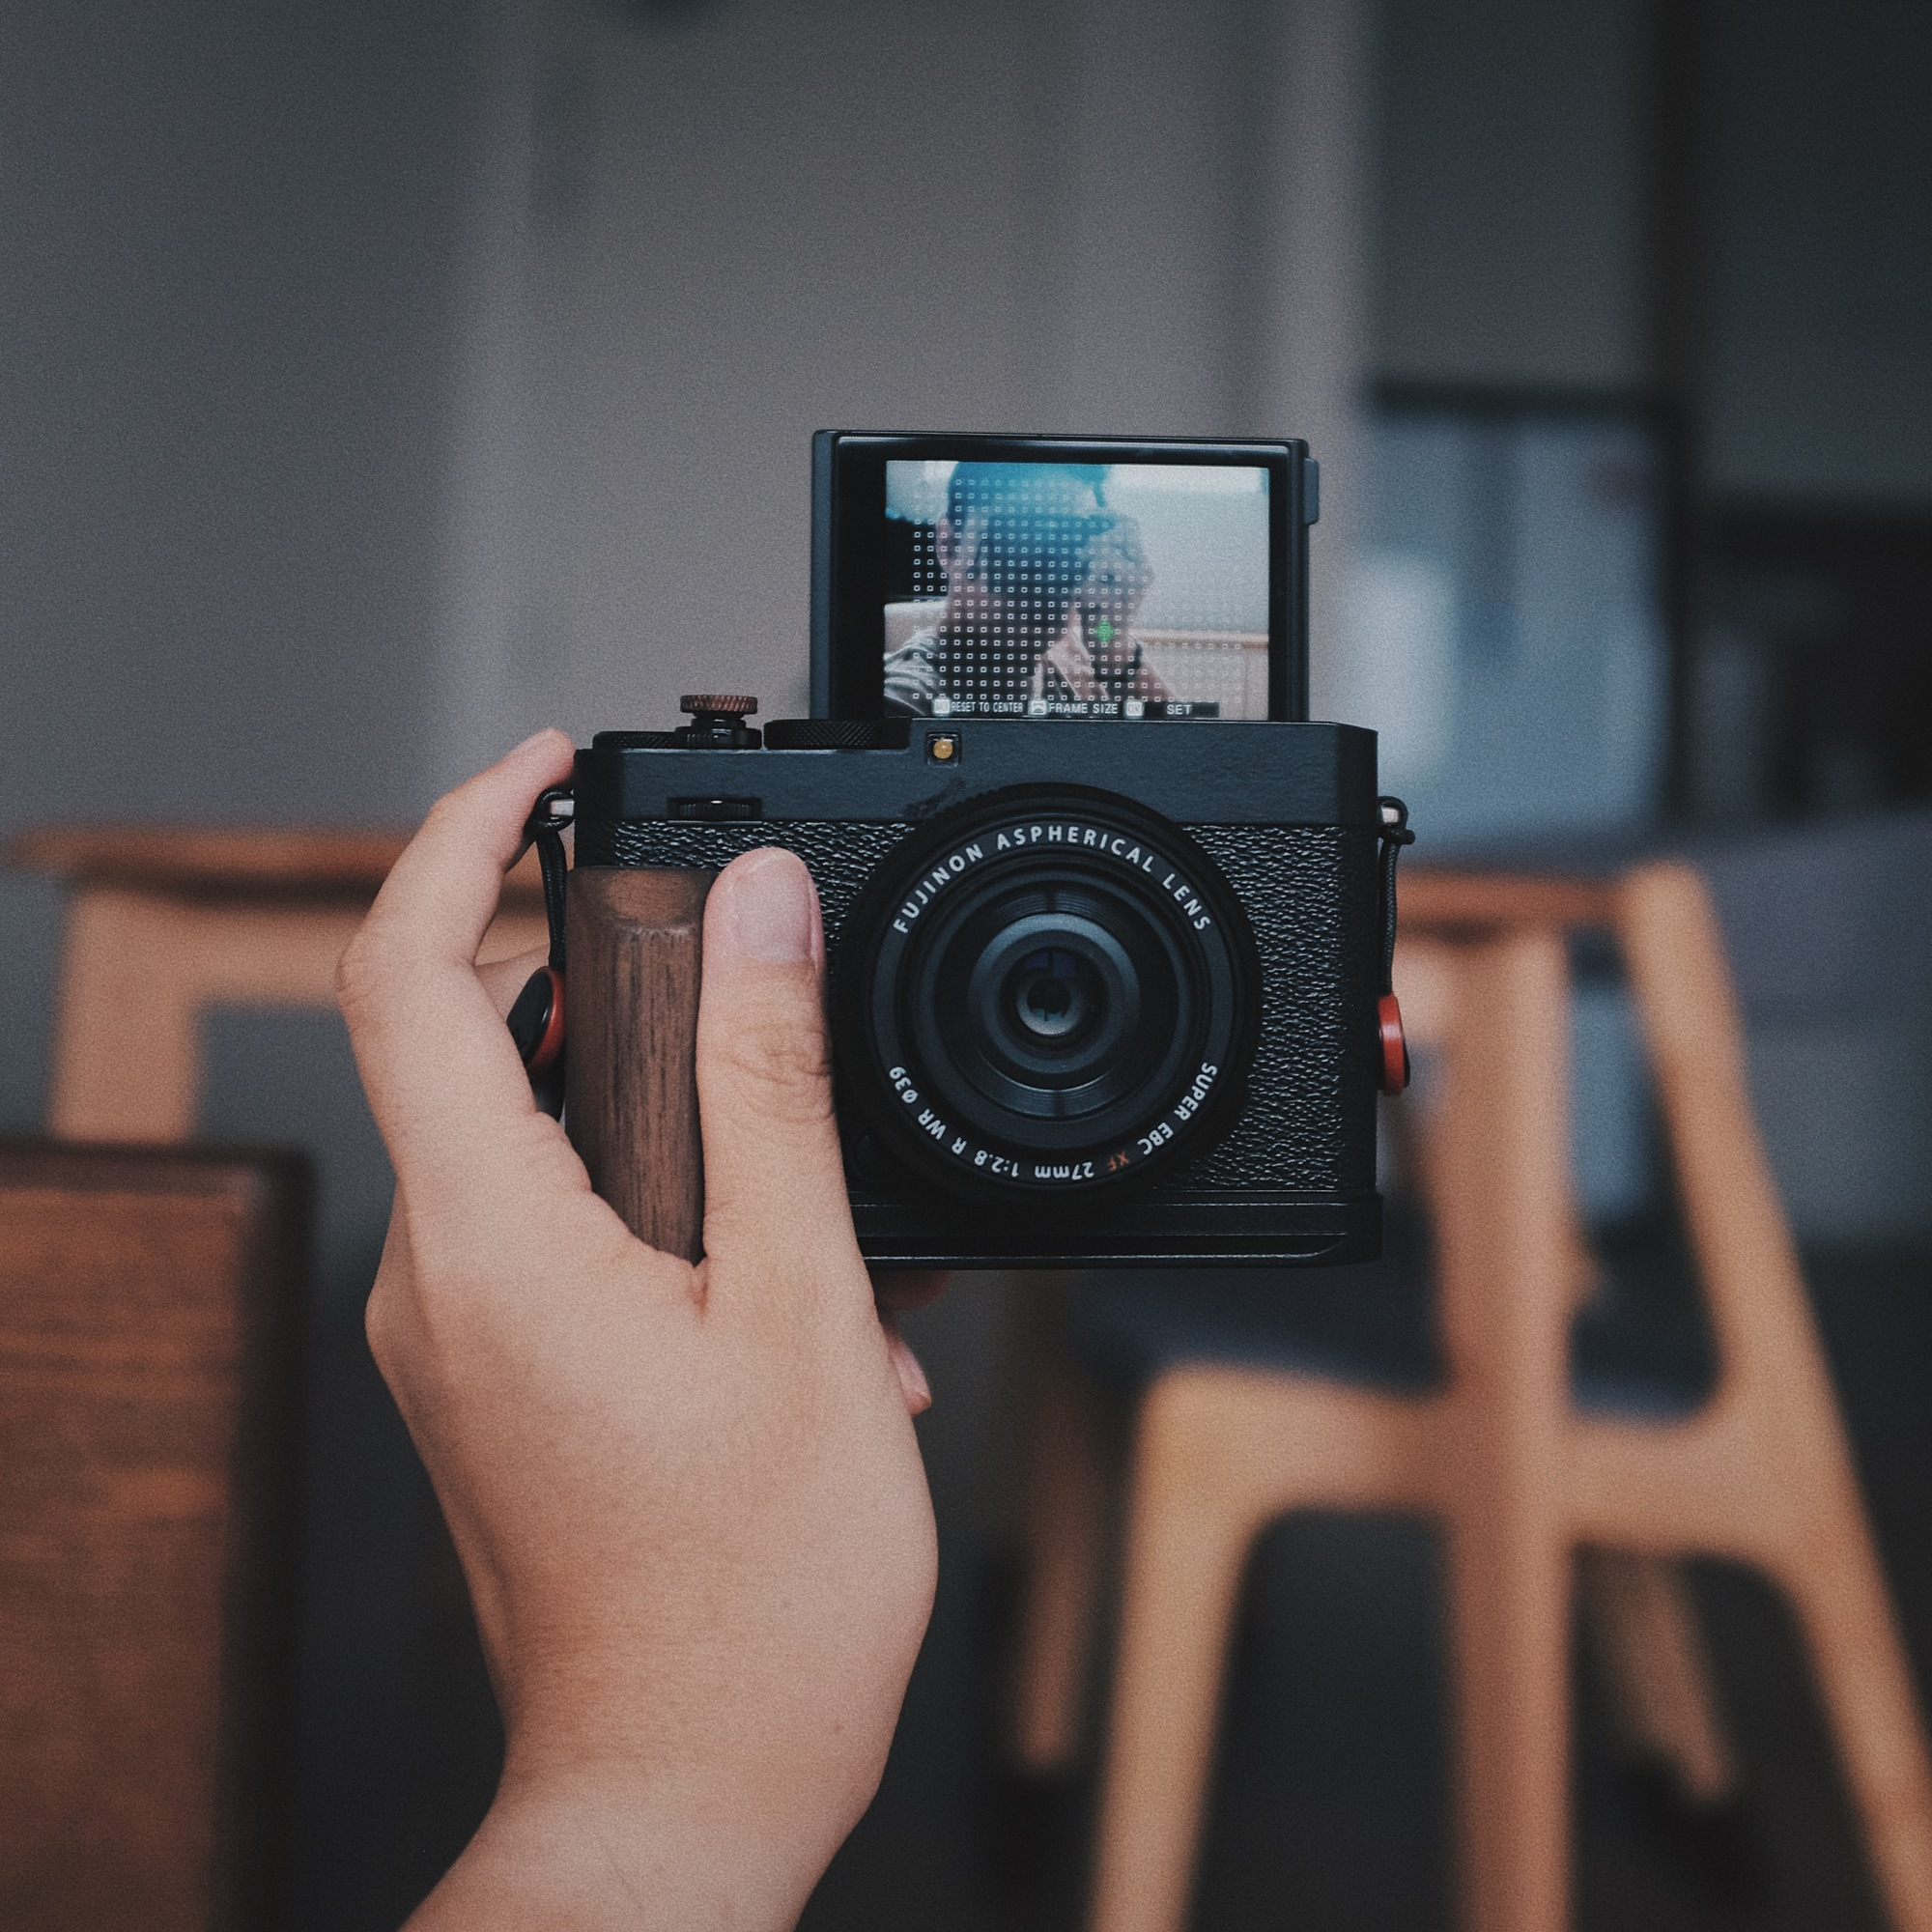
\includegraphics[width=\linewidth]{\envfinaldir/coverpic-prod.jpg}\par
            % \vskip 30pt
            \vfill

            \normalsize\rmfamily\scshape
            \copyright{} The Web Digest Project \hfill\large \envdatestr
        \end{center}
    \end{titlepage}
    % \restoregeometry
}
\newcommand{\simplehref}[1]{%
    \textcolor{blue!80!green}{\href{#1}{#1}}%
}
\renewcommand{\contentsname}{\center\Huge\sffamily\bfseries Contents\par\vskip 20pt}
\newcounter{ipartcounter}
\setcounter{ipartcounter}{0}
\newcommand{\ipart}[1]{
    % \vskip 20pt
    \clearpage
    \stepcounter{ipartcounter}
    \phantomsection
    \addcontentsline{toc}{chapter}{#1}
    % \begin{center}
    %     \Huge
    %     \sffamily\bfseries
    %     #1
    % \end{center}
    % \vskip 20pt plus 7pt
}
\newcounter{ichaptercounter}
\setcounter{ichaptercounter}{0}
\newcommand{\ichapter}[1]{
    % \vskip 20pt
    \clearpage
    \stepcounter{ichaptercounter}
    \phantomsection
    \addcontentsline{toc}{section}{\numberline{\arabic{ichaptercounter}}#1}
    \begin{center}
        \Huge
        \sffamily\bfseries
        #1
    \end{center}
    \vskip 20pt plus 7pt
}
\newcommand{\entrytitlefont}[1]{\subsection*{\raggedright\Large\sffamily\bfseries#1}}
\newcommand{\entryitemGeneric}[2]{
    % argv: title, url
    \parbox{\linewidth}{
        \entrytitlefont{#1}\par\vskip 5pt
        \footnotesize\ttfamily\mdseries
        \simplehref{#2}
    }\vskip 11pt plus 11pt minus 1pt
}
\newcommand{\entryitemGithub}[3]{
    % argv: title, url, desc
    \parbox{\linewidth}{
        \entrytitlefont{#1}\par\vskip 5pt
        \footnotesize\ttfamily\mdseries
        \simplehref{#2}\par\vskip 5pt
        \small\rmfamily\mdseries#3
    }\vskip 11pt plus 11pt minus 1pt
}
\newcommand{\entryitemAp}[3]{
    % argv: title, url, desc
    \parbox{\linewidth}{
        \entrytitlefont{#1}\par\vskip 5pt
        \footnotesize\ttfamily\mdseries
        \simplehref{#2}\par\vskip 5pt
        \small\rmfamily\mdseries#3
    }\vskip 11pt plus 11pt minus 1pt
}
\newcommand{\entryitemHackernews}[3]{
    % argv: title, hnurl, rawurl
    % \parbox{\linewidth}{
    %     \entrytitlefont{#1}\par\vskip 5pt
    %     \footnotesize\ttfamily\mdseries
    %     \simplehref{#3}\par
    %     \textcolor{black!50}{\href{#2}{#2}}
    % }\vskip 11pt plus 11pt minus 1pt
    \begin{minipage}{\linewidth}
            \entrytitlefont{#1}\par\vskip 5pt
            \footnotesize\ttfamily\mdseries
            \simplehref{#3}\par
            \textcolor{black!50}{\href{#2}{#2}}
    \end{minipage}\par\vskip 11pt plus 11pt minus 1pt
}







\begin{document}

\makeheader

\tableofcontents\clearpage




\ipart{Developers}
\ichapter{Hacker News}
\entryitemTwoLinks{A Letter to the American People}{https://news.ycombinator.com/item?id=43224350}{https://18f.org/}

\entryitemTwoLinks{GLP-1 drugs: An economic disruptor? (2024)}{https://news.ycombinator.com/item?id=43222791}{https://wildfirelabs.substack.com/p/the-100-trillion-disruption-the-unforeseen}

\entryitemTwoLinks{Making o1, o3, and Sonnet 3.7 hallucinate for everyone}{https://news.ycombinator.com/item?id=43222027}{https://bengarcia.dev/making-o1-o3-and-sonnet-3-7-hallucinate-for-everyone}

\entryitemTwoLinks{The most unhinged video wall, made out of Chromebooks}{https://news.ycombinator.com/item?id=43221697}{https://varun.ch/posts/videowall/}

\entryitemTwoLinks{GSA Eliminates 18F}{https://news.ycombinator.com/item?id=43221549}{https://www.nextgov.com/people/2025/03/gsa-eliminates-18f/403400/}

\entryitemTwoLinks{Copilot for Everything: Training your AI replacement one keystroke at a time}{https://news.ycombinator.com/item?id=43220938}{https://substack.com/home/post/p-158101095}

\entryitemTwoLinks{Become a sponsor to Servo}{https://news.ycombinator.com/item?id=43219865}{https://github.com/sponsors/servo}

\entryitemTwoLinks{Intel delays \$28B Ohio chip fabs to 2030}{https://news.ycombinator.com/item?id=43218915}{https://www.reuters.com/technology/intel-delays-28-billion-ohio-chip-factory-2030-local-media-reports-2025-02-28/}

\entryitemTwoLinks{GrapheneOS blocked exploitation of 3 Android zero-days used by Cellebrite}{https://news.ycombinator.com/item?id=43218872}{https://grapheneos.social/@GrapheneOS/114081753914226921}

\entryitemTwoLinks{A DOGE staffer appears to be posting DOGE work on his public GitHub}{https://news.ycombinator.com/item?id=43217947}{https://twitter.com/SollenbergerRC/status/1895609294810464390}

\entryitemTwoLinks{Yes, Claude Code can decompile itself. Here's the source code}{https://news.ycombinator.com/item?id=43217357}{https://ghuntley.com/tradecraft/}

\entryitemTwoLinks{Zen 5's AVX-512 Frequency Behavior}{https://news.ycombinator.com/item?id=43215781}{https://chipsandcheese.com/p/zen-5s-avx-512-frequency-behavior}

\entryitemTwoLinks{When eBPF pt\_regs reads return garbage on the latest Linux kernels, blame Fred}{https://news.ycombinator.com/item?id=43214576}{https://tanelpoder.com/posts/ebpf-pt-regs-error-on-linux-blame-fred/}

\entryitemTwoLinks{Self-Hosting a Firefox Sync Server}{https://news.ycombinator.com/item?id=43214294}{https://blog.diego.dev/posts/firefox-sync-server/}

\entryitemTwoLinks{The housing theory of everything (2021)}{https://news.ycombinator.com/item?id=43214263}{https://worksinprogress.co/issue/the-housing-theory-of-everything/}

\entryitemTwoLinks{An update on Mozilla's terms of use for Firefox}{https://news.ycombinator.com/item?id=43213612}{https://blog.mozilla.org/en/products/firefox/update-on-terms-of-use/}

\entryitemTwoLinks{Inheriting is becoming nearly as important as working}{https://news.ycombinator.com/item?id=43213143}{https://www.economist.com/leaders/2025/02/27/inheriting-is-becoming-nearly-as-important-as-working}

\entryitemTwoLinks{Why it's so hard to build a jet engine}{https://news.ycombinator.com/item?id=43212952}{https://www.construction-physics.com/p/why-its-so-hard-to-build-a-jet-engine}

\entryitemTwoLinks{Brian Krebs: This Administration Is Completely Compromised}{https://news.ycombinator.com/item?id=43211506}{https://infosec.exchange/@briankrebs/114083485241630234}

\entryitemTwoLinks{How to gain code execution on hundreds of millions of people and popular apps}{https://news.ycombinator.com/item?id=43210858}{https://kibty.town/blog/todesktop/}\ichapter{Phoronix}
\entryitemGeneric{\hskip 0pt{}Linux's New Way Of Informing User-Space Over Hung GPUs May Become More Useful}{https://www.phoronix.com/news/Extending-Linux-GPU-Wedge-Event}

\entryitemGeneric{\hskip 0pt{}AMD Readies More Graphics Driver Improvements For Linux 6.15}{https://www.phoronix.com/news/AMDGPU-Linux-6.15-Round-2}

\entryitemGeneric{\hskip 0pt{}Intel Core 2 CPUs Have Been Affected By An Annoying Linux Kernel Bug For 5+ Years}{https://www.phoronix.com/news/Intel-Core-2-Stalls-Boot-Fix}

\entryitemGeneric{\hskip 0pt{}NVIDIA Blackwell, Continued AMD Zen 5 Benchmarking \& Rust Drama Dominated February}{https://www.phoronix.com/news/February-2025-Highlights}

\entryitemGeneric{\hskip 0pt{}GNOME's Mutter Now Supports The Wayland Cursor Shape Protocol}{https://www.phoronix.com/news/GNOME-Mutter-Cursor-Shape}

\entryitemGeneric{\hskip 0pt{}KDE Developers Begin More Feature Work On Plasma 6.4}{https://www.phoronix.com/news/KDE-Plasma-6.4-Past-6.3}

\entryitemGeneric{\hskip 0pt{}DeepSeek Develops Linux File-System For Better AI Training \& Inference Performance}{https://www.phoronix.com/news/DeekSeek-3FS-File-System}

\entryitemGeneric{\hskip 0pt{}NVIDIA Vulkan Beta Driver Updated For Blackwell \& New Extensions}{https://www.phoronix.com/news/NVIDIA-Vulkan-Beta-EO-Feb-2025}

\entryitemGeneric{\hskip 0pt{}AMD Prepares Linux Driver Support For Image Signal Processor With New Laptops}{https://www.phoronix.com/news/AMD-ISP4-Linux-Laptop-Driver}


\ipart{Developers~~~~(zh-Hans)}
\ichapter{V2EX}
\entryitemGeneric{\hskip 0pt{}[问与答] 客服类大模型}{https://www.v2ex.com/t/1115179}

\entryitemGeneric{\hskip 0pt{}[问与答] 独立站 cf 安全设置}{https://www.v2ex.com/t/1115178}

\entryitemGeneric{\hskip 0pt{}[职场话题] 询问 408 考研如今如何?是否有必要转其他专业?比如通信工程}{https://www.v2ex.com/t/1115177}

\entryitemGeneric{\hskip 0pt{}[分享创造] 开发了一个分享文件的玩具-FileBox}{https://www.v2ex.com/t/1115175}

\entryitemGeneric{\hskip 0pt{}[Apple] 心痒痒 m4 macmini,该不该冲动消费?}{https://www.v2ex.com/t/1115174}

\entryitemGeneric{\hskip 0pt{}[前端开发] react 是一个库, vue 是一个框架,所以 react 牛批}{https://www.v2ex.com/t/1115173}

\entryitemGeneric{\hskip 0pt{}[宠物] 江浙沪买猫。女朋友闹着要猫,短腿起司猫那种的,求个靠谱渠道,可自提}{https://www.v2ex.com/t/1115172}

\entryitemGeneric{\hskip 0pt{}[Apple] 现在入手 Apple tv7 代合适吗?}{https://www.v2ex.com/t/1115171}

\entryitemGeneric{\hskip 0pt{}[分享创造] 现在还有人玩 2048 小游戏吗,做了一个在线玩 2048 的游戏站。 主打一个无广告,纯公益 ………… https://2048juego.com}{https://www.v2ex.com/t/1115169}

\entryitemGeneric{\hskip 0pt{}[iCloud] 有没有那种通知 iCloud 国区充值优惠的频道/公众号之类的?}{https://www.v2ex.com/t/1115168}

\entryitemGeneric{\hskip 0pt{}[云计算] 求推荐便宜可靠的图片内容安全检测服务}{https://www.v2ex.com/t/1115167}

\entryitemGeneric{\hskip 0pt{}[问与答] 如何从视频中提取特定的几何图像}{https://www.v2ex.com/t/1115166}

\entryitemGeneric{\hskip 0pt{}[分享发现] 始祖鸟居然是安踏的}{https://www.v2ex.com/t/1115165}

\entryitemGeneric{\hskip 0pt{}[程序员] 使用 AI 编程体验和一些想法}{https://www.v2ex.com/t/1115163}

\entryitemGeneric{\hskip 0pt{}[分享发现] Follow 公测了}{https://www.v2ex.com/t/1115162}

\entryitemGeneric{\hskip 0pt{}[问与答] 问一下现在中国大陆好用的静态资源库还有什么?}{https://www.v2ex.com/t/1115161}

\entryitemGeneric{\hskip 0pt{}[VMware] 博通网站上的 VMware Workstation 下载地址没了?}{https://www.v2ex.com/t/1115160}

\entryitemGeneric{\hskip 0pt{}[程序员] 想问下大佬生成 UI 页面的工具哪个好}{https://www.v2ex.com/t/1115158}

\entryitemGeneric{\hskip 0pt{}[Apple] Mac mini 配置清单}{https://www.v2ex.com/t/1115156}

\entryitemGeneric{\hskip 0pt{}[macOS] macos 15 也太垃圾了}{https://www.v2ex.com/t/1115154}

\entryitemGeneric{\hskip 0pt{}[问与答] 🔴v2rayNG 自动更新订阅后必须手动激活的问题?🔴}{https://www.v2ex.com/t/1115153}

\entryitemGeneric{\hskip 0pt{}[程序员] 我又以程序员的思维做了个开发全家通的导航站-基于 CMMI3 的流程分类。不知道能不能行}{https://www.v2ex.com/t/1115151}

\entryitemGeneric{\hskip 0pt{}[职场话题] 警惕 AI 对我们的影响,}{https://www.v2ex.com/t/1115148}

\entryitemGeneric{\hskip 0pt{}[酷工作] [付费咨询] 求一名移动端应用 UI 资深设计师,按时付费}{https://www.v2ex.com/t/1115147}

\entryitemGeneric{\hskip 0pt{}[问与答] 各位大佬在家里的树莓派都干什么用的?}{https://www.v2ex.com/t/1115144}

\entryitemGeneric{\hskip 0pt{}[Apple] macOS 锁屏界面按下 esc 息屏后立刻亮屏再次进入锁屏界面,请问如何解决?}{https://www.v2ex.com/t/1115143}

\entryitemGeneric{\hskip 0pt{}[问与答] 买 ThinkBook 该如何抉择?}{https://www.v2ex.com/t/1115141}

\entryitemGeneric{\hskip 0pt{}[Python] 初学 fleet,请问如何实现自动补完和开启错误提示?}{https://www.v2ex.com/t/1115140}

\entryitemGeneric{\hskip 0pt{}[macOS] 为什么 macOS 至今不支持对 Chrome 等非 quickTime 解码器的音频播放器开启 AirPods 空间音频?我用 VLC 写了个 Demo, iOS 这种系统没有二次混音都支持,不开 AirPods 感觉音质很糊}{https://www.v2ex.com/t/1115139}

\entryitemGeneric{\hskip 0pt{}[NAS] 求助帖,群晖 synology photos 不识别 live photos 了}{https://www.v2ex.com/t/1115138}

\entryitemGeneric{\hskip 0pt{}[问与答] 求可 selfhost 的书签生成浏览器起始页的插件或项目}{https://www.v2ex.com/t/1115136}

\entryitemGeneric{\hskip 0pt{}[宽带症候群] 上海联通单宽带说是企业宽带靠谱吗}{https://www.v2ex.com/t/1115135}

\entryitemGeneric{\hskip 0pt{}[问与答] iPhone 17 会全部取消使用 MagSafe 吗?}{https://www.v2ex.com/t/1115134}

\entryitemGeneric{\hskip 0pt{}[宽带症候群] 几年没用 NTT 线路 联通现在这么好了?}{https://www.v2ex.com/t/1115131}

\entryitemGeneric{\hskip 0pt{}[Apple] 为了 apple intelligence,换账号, 换出大麻烦了}{https://www.v2ex.com/t/1115130}

\entryitemGeneric{\hskip 0pt{}[分享创造] 对本站之前看到的一个小项目 DenoProxy 进行了增强}{https://www.v2ex.com/t/1115128}

\entryitemGeneric{\hskip 0pt{}[上海] 有没有线下交流一下投资的?}{https://www.v2ex.com/t/1115127}

\entryitemGeneric{\hskip 0pt{}[YouTube] 油管的工程师在搞什么飞机}{https://www.v2ex.com/t/1115126}

\entryitemGeneric{\hskip 0pt{}[生活] 水管漏水, 计算后, 我不需要补了}{https://www.v2ex.com/t/1115125}

\entryitemGeneric{\hskip 0pt{}[远程工作] [远程兼职] 求一名硬件产品经理,线上兼职 , 300/时}{https://www.v2ex.com/t/1115124}

\entryitemGeneric{\hskip 0pt{}[推广] 一个 VPS 推介站,主机啦}{https://www.v2ex.com/t/1115123}

\entryitemGeneric{\hskip 0pt{}[程序员] 求问下 v 友们一个物联网开发问题}{https://www.v2ex.com/t/1115122}

\entryitemGeneric{\hskip 0pt{}[加密货币] 加密货币量化机器人 banbot,带策略,欢迎有编程基础的尝试}{https://www.v2ex.com/t/1115121}

\entryitemGeneric{\hskip 0pt{}[职场话题] [工资流水] 请问在职打印工资流水有什么风险吗}{https://www.v2ex.com/t/1115120}

\entryitemGeneric{\hskip 0pt{}[路由器] 求推荐款性能功能不错的家用路由器}{https://www.v2ex.com/t/1115119}

\entryitemGeneric{\hskip 0pt{}[生活] 谈了快 10 年的女朋友要求 30 万彩礼}{https://www.v2ex.com/t/1115118}

\entryitemGeneric{\hskip 0pt{}[ThinkPad] 换电池有推荐}{https://www.v2ex.com/t/1115117}

\entryitemGeneric{\hskip 0pt{}[问与答] 微信公众号,用户上传图片怎么最大限度避免违规?求经验}{https://www.v2ex.com/t/1115116}

\entryitemGeneric{\hskip 0pt{}[问与答] Cursor 如何付费}{https://www.v2ex.com/t/1115115}

\entryitemGeneric{\hskip 0pt{}[macOS] ImageThumbnailExtension 是什么?}{https://www.v2ex.com/t/1115113}


\ipart{Generic News}







\clearpage
\leavevmode\vfill
\footnotesize

Copyright \copyright{} 2023-2025 Neruthes and other contributors.

This document is published with CC BY-NC-ND 4.0 license.

The entries listed in this newsletter may be copyrighted by their respective creators.

This newsletter is generated by the Web Digest project.

The newsletters are also delivered via Telegram channel \CJKunderline{\href{https://t.me/webdigestchannel}{https://t.me/webdigestchannel}}.\\
RSS feed is available at \CJKunderline{\href{https://webdigest.pages.dev/rss.xml}{https://webdigest.pages.dev/rss.xml}}.

This newsletter is available in PDF at
\CJKunderline{\href{https://webdigest.pages.dev/}{https://webdigest.pages.dev/}}.

The source code being used to generate this newsletter is available at\\
\CJKunderline{\href{https://github.com/neruthes/webdigest}{https://github.com/neruthes/webdigest}}.

This newsletter is also available in
\CJKunderline{\href{http://webdigest.pages.dev/readhtml/\envyear/WebDigest-20250302.html}{HTML}} and
\CJKunderline{\href{https://github.com/neruthes/webdigest/blob/master/markdown/\envyear/WebDigest-20250302.md}{Markdown}}.


\coverpic{https://unsplash.com/photos/a-tall-palm-tree-sitting-in-front-of-a-tall-building-5Wx4qyjdtq0}{Lena Polishko}


\end{document}
